%% 11/23/2015
%%%%%%%%%%%%%%%%%%%%%%%%%%%%%%%%%%%%%%%%%%%%%%%%%%%%%%%%%%%%%%%%%%%%%%%%%%%%
% AGUJournalTemplate.tex: this template file is for articles formatted with LaTeX
%
% This file includes commands and instructions
% given in the order necessary to produce a final output that will
% satisfy AGU requirements. 
%
% You may copy this file and give it your
% article name, and enter your text.
%
%%%%%%%%%%%%%%%%%%%%%%%%%%%%%%%%%%%%%%%%%%%%%%%%%%%%%%%%%%%%%%%%%%%%%%%%%%%%
% PLEASE DO NOT USE YOUR OWN MACROS
% DO NOT USE \newcommand, \renewcommand, or \def, etc.
%
% FOR FIGURES, DO NOT USE \psfrag or \subfigure.
% DO NOT USE \psfrag or \subfigure commands.
%%%%%%%%%%%%%%%%%%%%%%%%%%%%%%%%%%%%%%%%%%%%%%%%%%%%%%%%%%%%%%%%%%%%%%%%%%%%
%
% Step 1: Set the \documentclass
%
% There are two options for article format:
%
% 1) PLEASE USE THE DRAFT OPTION TO SUBMIT YOUR PAPERS.
% The draft option produces double spaced output.
% 
% 2) numberline will give you line numbers.

%% To submit your paper:
\documentclass[draft, linenumbers]{agujournal}
%\draftfalse

%% For final version.
% \documentclass{agujournal}

% Now, type in the journal name: \journalname{<Journal Name>}

% ie, \journalname{Journal of Geophysical Research}
%% Choose from this list of Journals:
%
% JGR-Atmospheres
% JGR-Biogeosciences
% JGR-Earth Surface
% JGR-Oceans
% JGR-Planets
% JGR-Solid Earth
% JGR-Space Physics
% Global Biochemical Cycles
% Geophysical Research Letters
% Paleoceanography
% Radio Science
% Reviews of Geophysics
% Tectonics
% Space Weather
% Water Resource Research
% Geochemistry, Geophysics, Geosystems
% Journal of Advances in Modeling Earth Systems (JAMES)
% Earth's Future
% Earth and Space Science
%
%

\journalname{Geophysical Research Letters}


\begin{document}

%% ------------------------------------------------------------------------ %%
%  Title
% 
% (A title should be specific, informative, and brief. Use
% abbreviations only if they are defined in the abstract. Titles that
% start with general keywords then specific terms are optimized in
% searches)
%
%% ------------------------------------------------------------------------ %%

% Example: \title{This is a test title}

\title{Microburst Scale Size Derived from Multiple Bounces of a Microburst Simultaneously Observed with the FIREBIRD-II CubeSats}

%% ------------------------------------------------------------------------ %%
%
%  AUTHORS AND AFFILIATIONS
%
%% ------------------------------------------------------------------------ %%

% Authors are individuals who have significantly contributed to the
% research and preparation of the article. Group authors are allowed, if
% each author in the group is separately identified in an appendix.)

% List authors by first name or initial followed by last name and
% separated by commas. Use \affil{} to number affiliations, and
% \thanks{} for author notes.  
% Additional author notes should be indicated with \thanks{} (for
% example, for current addresses). 

% Example: \authors{A. B. Author\affil{1}\thanks{Current address, Antartica}, B. C. Author\affil{2,3}, and D. E.
% Author\affil{3,4}\thanks{Also funded by Monsanto.}}

\authors{Mykhaylo Shumko\affil{1}, John Sample\affil{1}, Arlo Johnson\affil{1}, Bern Blake\affil{2}, Alex Crew\affil{3}, Harlan Spence\affil{4}, David Klumpar\affil{1}, Oleksiy Agapitov\affil{5}, Matthew Handley\affil{1}}

\affiliation{1}{Department of Physics, Montana State University, Bozeman, Montana, USA}
\affiliation{2}{Space Science Applications Laboratory, The Aerospace Corporation, Los Angeles, California, USA}
\affiliation{3}{The Johns Hopkins University Applied Physics Laboratory LLC, Laurel, Maryland, USA}
\affiliation{4}{Institute for the Study of Earth, Oceans, and Space, University of New Hampshire, Durham, New Hampshire, USA}
\affiliation{5}{Space Sciences Laboratory, UC Berkeley, Berkeley, California, USA}


%% Corresponding Author:
% Corresponding author mailing address and e-mail address:

% (include name and email addresses of the corresponding author.  More
% than one corresponding author is allowed in this LaTeX file and for
% publication; but only one corresponding author is allowed in our
% editorial system.)  

% Example: \correspondingauthor{First and Last Name}{email@address.edu}

\correspondingauthor{Mykhaylo Shumko}{msshumko@gmail.com}

%% Keypoints, final entry on title page.

% Example: 
% \begin{keypoints}
% \item	List up to three key points (at least one is required)
% \item	Key Points summarize the main points and conclusions of the article
% \item	Each must be 100 characters or less with no special characters or punctuation 
% \end{keypoints}

%  List up to three key points (at least one is required)
%  Key Points summarize the main points and conclusions of the article
%  Each must be 100 characters or less with no special characters or punctuation 

\begin{keypoints}
\item Multiple bounces from a microburst were observed by two FIREBIRD-II CubSats at LEO.
\item The lower bounds on the microburst scale size at LEO were $29 \pm 1$ km (latitudinal) and $51 \pm 11$ km (longitudinal).
\item Deduced lower bound equatorial scale size was similar to the whistler-mode chorus source scale.
\end{keypoints}

%% ------------------------------------------------------------------------ %%
%
%  ABSTRACT
%
% A good abstract will begin with a short description of the problem
% being addressed, briefly describe the new data or analyses, then
% briefly states the main conclusion(s) and how they are supported and
% uncertainties. 
%% ------------------------------------------------------------------------ %%

%% \begin{abstract} starts the second page 

\begin{abstract}
We present the observation of a spatially large microburst with multiple bounces made simultaneously by the FIREBIRD-II CubeSats on February 2nd, 2015. This is the first observation of a microburst with a subsequent decay made by two co-orbiting but spatially separated spacecraft. From these unique measurements, we place estimates on the lower bounds of the spatial scales as well as quantify the electron bounce periods. The microburst's lower bound latitudinal scale size was $29 \pm 1$ km and the longitudinal scale size was $51 \pm 1$  km in low earth orbit. We mapped these scale sizes to the magnetic equator and found that the radial and azimuthal scale sizes were at least $500 \pm​ 10$ km and $530 \pm 10$ km, respectively. These lower bound equatorial scale sizes are similar to whistler-mode chorus wave source scale sizes, which supports the hypothesis that microbursts are a product of electron scattering by chorus waves. Lastly, we estimated the bounce periods for 200-800 keV electrons and found good agreement with four common magnetic field models.
\end{abstract}
%% ------------------------------------------------------------------------ %%
%
%  TEXT
%
%% ------------------------------------------------------------------------ %%

%%% Suggested section heads:
% \section{Introduction}
% 
% The main text should start with an introduction. Except for short
% manuscripts (such as comments and replies), the text should be divided
% into sections, each with its own heading. 

% Headings should be sentence fragments and do not begin with a
% lowercase letter or number. Examples of good headings are:

% \section{Materials and Methods}
% Here is text on Materials and Methods.
%
% \subsection{A descriptive heading about methods}
% More about Methods.
% 
% \section{Data} (Or section title might be a descriptive heading about data)
% 
% \section{Results} (Or section title might be a descriptive heading about the
% results)
% 
% \section{Conclusions}

\section{Introduction}\label{Intro}
% use \citet for direct references, \citep for indirect.
The dynamics of radiation belt electrons are complex, and are driven by competition between source and loss processes. A few possible loss processes are radial diffusion \citep{Shprits2004}, magnetopause shadowing \citep{Ukhorskiy2006}, and pitch angle and energy diffusion due to scattering of electrons by plasma waves \citep[e.g.][]{Abel1998_1, Summers1998, Meredith2002, Selesnick2003, Horne2003, Thorne2005, Mozer2018}. There are a variety of waves that cause pitch angle scattering, including electromagnetic ion cyclotron waves, plasmaspheric hiss, and chorus \citep{Millan2007, Thorne2010}. Chorus predominantly occurs in the dawn sector (6-12 magnetic local times (MLT)) \citep{Li2009} where it accelerates electrons with large equatorial pitch angles and scatters electrons with small equatorial pitch angles \citep{Horne2003}. Some of these electrons may be impulsively scattered into the loss cone, where they result in short-duration ($\sim 100$ ms) enhancements in precipitating flux called microbursts.

\citet{Anderson1964} coined the term microburst to describe high altitude balloon observations of $\sim 100$ ms duration enhancements of bremsstrahlung X-rays emitted from scattered microburst electrons impacting the atmosphere. Since then, non-relativistic (less than a few hundred keV) microbursts have been routinely observed with other balloon missions \citep[e.g.][]{Parks1967, Woodger2015, Anderson2017}. A review of the literature shows no reports of microbursts above a few hundred keV observed by balloons \citep{Millan2002, Woodger2015}. This lack of observation may be explained by relatively weaker pitch angle scattering of relativistic electrons by chorus \citep{Lee2012}. 

In addition to the X-ray signature proxy for bursts of electron precipitation, the precipitating relativistic and non-relativistic electrons have been measured in situ by spacecraft orbiting in low earth orbit (LEO). Hereinafter, we refer to these electron signatures observed by LEO spacecraft also as microbursts. Microbursts have been observed with, e.g. the Solar Anomalous and Magnetospheric Particle Explorer's (SAMPEX) > 150 keV and > 1 MeV channels \citep{Nakamura1995, Nakamura2000, Blake1996, Lorentzen2001a, Lorentzen2001b, O'Brien2003, O'Brien2004, Blum2015} and Focused Investigation of Relativistic Electron Bursts: Intensity, Range, and Dynamics (FIREBIRD-II) with its > 200 keV energy channels \citep{Crew2016, Anderson2017, Breneman2017}. \deleted{To characterize the source of microbursts, \textit{Lorentzen et al.,} 2001 found that microbursts and chorus waves predominantly occur in the dawn sector and \textit{Breneman et al.,} 2017 made a direct observational link between individual microbursts and chorus elements.}

\added{Understanding microburst precipitation and its scattering mechanism is important to radiation belt dynamics. Microbursts have been modeled and empirically estimated to be capable of depleting the relativistic electron population in the outer radiation belt on the order of a day \citep{O'Brien2004, Thorne2005, Shprits2007, Breneman2017}. The scattering mechanism has been observatioanlly studied by e.g. \citet{Lorentzen2001b} who found that microbursts and chorus waves predominantly occur in the dawn sector and \citet{Breneman2017} made a direct observational link between individual microbursts and chorus elements.} An important parameter in this estimation of instantaneous radiation belt electron losses due to microbursts is their scale size. \citet{Parks1967} used balloon measurements of bremsstrahlung X-rays to estimate the high altitude scale size of predominantly low energy microbursts to be $40 \pm 14$ km. In \citet{Blake1996} a microburst with multiple bounces was observed by SAMPEX, and the microburst's latitudinal scale size in LEO was estimated to have been ``at least a few tens of kilometers". \citet{Blake1996} concluded that typically microbursts are less than a few tens of electron gyroradii in size (at L = 5 at LEO, the gyroradii of 1 MeV electrons is on the order of 100 m). \citet{Dietrich2010} used SAMPEX along with ground-based very low frequency stations to conclude that during one SAMPEX pass, the observed microbursts had scale sizes less than $4$ km.

Since February 1st, 2015, microbursts have been observed by FIREBIRD-II, a pair of CubeSats in LEO. Soon after launch, when the two FIREBIRD-II spacecraft were at close range, a microburst with a scale size greater than 11 km was observed \citep{Crew2016}. On the same day, FIREBIRD-II simultaneously observed a microburst with multiple bounces. The microburst decay was observed over a period of a few seconds, while the spacecraft were traveling predominantly in latitude. Here we present the analysis and results of the latitude and longitude scale sizes and bounce periods of the first microburst with multiple bounces observed with the two FIREBIRD-II spacecraft.

\section{Spacecraft and Observation} \label{obs} %%%%%%%%%%%%%%%%%%%%%%%%%%%%%%%%%%%%%%%%%%%%%%%%%%%%%%%%%%%%%%%%%%%%%%%%%%
The FIREBIRD missions are comprised of a pair of identically-instrumented 1.5U CubeSats (15 x 10 x 10 cm) that are designed to measure electron precipitation in LEO \citep{Spence2012, Klumpar2015}. The second mission, termed FIREBIRD-II, was launched on January 31st 2015.  The two FIREBIRD-II CubeSats, identified as Flight Unit 3 (FU3) and Flight Unit 4 (FU4), were placed \added{in a} 632 km apogee, 433 km perigee, and $99^{\circ}$ inclination orbit \citep{Crew2016}. FU3 and FU4 are orbiting in a string of pearls configuration with FU4 ahead, to resolve the space-time ambiguity of \replaced{events}{microbursts.} \deleted{that are either spatial or temporal.} Each FIREBIRD-II unit has two solid state detectors: one is mounted essentially at the spacecraft surface, covered only by a thin foil acting as a sun shade, with a field of view of $90^{\circ}$ (surface detector), and the other is beneath a collimator which restricts the field of view to $54^{\circ}$ (collimated detector). Only FU3 has a functioning surface detector, so this analysis utilizes the collimated detectors. FU3's surface and collimated detectors, as well as FU4's collimated detector observe electron fluxes in six energy channels from $\sim 230$ keV to $> 1$ MeV. \added{FIREBIRD-II's High Resolution (HiRes) electron flux data is gathered} with an adjustable sampling \replaced{rate}{period} of 18.75 ms by default and as fast as 12.5 ms. 

On February 2nd, 2015 at 06:12 UT, both FIREBIRD-II spacecraft simultaneously observed an initial microburst, followed by subsequent periodic electron enhancements of diminishing amplitude shown in Fig. \ref{hires_plot}. This is thought to be the signature of a single burst of electrons, some of which precipitate, but the rest mirror near the spacecraft then bounce to the conjugate hemisphere where they mirror again. \added{As a result, the subsequent bounces} produce a train of decaying peaks \citep{Blake1996, Thorne2005}. This bounce signature occurred during the transition between the main and recovery phases of a storm with a minimum Dst of -44 nT (Kp = 4, and AE ${\approx 400}$ nT). At this time, the \replaced{High Resolution (HiRes) electron flux}{HiRes data} was sampled at 18.75 ms. Five peaks were observed by both spacecraft. The fifth peak observed by FU4 was comparable to the Poisson noise and was not used in this analysis. This microburst was observed from the first energy channel ($\approx 200-300$ keV), to the fourth energy channel ($\approx 500-700$ keV), and FU3's surface detector observed the microburst up to the fifth energy channel (683 - 950 keV). 

The HiRes data in Fig. \ref{hires_plot} shows signs of energy dispersion, characterized by higher energy electrons arriving earlier than the lower energies. This time of flight energy dispersion tends to smear out the initial sharp burst upon each subsequent bounce. The first peak does not appear to be dispersed, and subsequent peaks show a dispersion trend consistent across energy channels. The black vertical bars have been added to Fig. \ref{hires_plot} to highlight this energy dispersion. This dispersion signature and amplitude decay implies that the first peak was observed soon after the electrons were scattered, followed by decaying bounces.

At this time, in magnetic coordinates, FIREBIRD-II was at McIlwain L = 4.7 and MLT = 8.3, calculated with the Tsyganenko 1989 (T89) magnetic field model \citep{Tsyganenko1989} using IRBEM-Lib \citep{irbem}. Geographically, they were above Sweden, latitude = $63^{\circ}$N, longitude = $15^{\circ}$E, altitude = 650 km. This geographic location is magnetically conjugate to the east of the so-called South Atlantic Anomaly (SAA). The SAA is the location where the mirror points of electrons tend to occur at locations deeper in the atmosphere owing to the offset of the dipole magnetic field from the Earth's center. \replaced{Electrons that encounter the SAA are removed from their eastward longitudinal drift paths [\textit{Comess et al., 2003; Dietrich et al., 2010}]. This loss effect is termed the drift loss cone (DLC).}{Electrons with pitch angles within the drift loss cone (DLC) will encounter the SAA and be removed from their eastward longitudinal drift paths \citep{Comess2013, Dietrich2010}.} FU3 and FU4 are therefore both in regions where the particles in the DLC have recently precipitated, leaving only particles that were recently scattered. At the spacecraft location, locally mirroring electrons would have mirrored at 95 km in the opposite hemisphere, with more field aligned electrons mirroring at even lower altitudes. From the analysis done by \citet{Fang2010}, the peak in the total ionization rate in the atmosphere for 100 keV electrons is around 80 km altitude, while the total ionization rate from 1 MeV electrons peaks around 60 km altitude. It is, therefore, expected that a fraction of the microburst electrons will survive each encounter with the atmosphere. By plotting the peak flux as a function of bounce (not shown), it was found that 40 - 60 \% of the microburst electrons were lost on the first bounce, similar to the 33\% loss per bounce observed for a bouncing microburst observed by SAMPEX \citep{Thorne2005}.

\section{Analysis} \label{analysis} %%%%%%%%%%%%%%%%%%%%%%%%%%%%%%%%%%%%%%%%%%%%%%%%%%%%%%%%%%%%%%%%%%%%%%%%%%%%%%%%%%%%%%%%%
At the beginning of the FIREBIRD-II mission, two issues prevented the proper analysis of the microburst's spatial scale size: the spacecraft clocks were not synchronized, and their relative positions were not accurately known. We addressed these issues with a cross-correlation time lag analysis described in detail in the supporting information (SI). From this analysis, the time correction was $2.28 \pm 0.12$ s (applied to Fig. \ref{hires_plot}) and the separation was $19.9 \pm 0.9$ km at the time of the microburst observation.

\subsection{Electron Bounce Period} \label{t_b} %%%%%%%%%%%%%%%%%%%%%%%%%%%%%%%%%%%%%%%%%%%%%%%%%%%%%%%%%%%%%%%
We used this unique observation of bouncing electrons to calculate the bounce period, $t_b$ as a function of energy and compare it to $t_b$ derived from four magnetic field models, \added{the results of which are shown in Fig. \ref{tb_plot}}. The observed $t_b$ and uncertainties were calculated by fitting the baseline-subtracted HiRes flux. The baseline flux used in this analysis is given in \citet{O'Brien2004} as the flux at the 10th percentile over a specified time interval, which in this analysis was taken to be 0.5 seconds. The flux was fitted with a superposition of Gaussians for each energy channel, and the uncertainty in flux was calculated using the Poisson error from the microburst and baseline fluxes summed in quadrature. Using the fit parameters, the mean $t_b$ for the lowest four energy channels is shown in Fig. \ref{tb_plot}. The trend of decreasing $t_b$ as a function of energy is evident in Fig. \ref{tb_plot}, which further supports the assumption that the subsequent peaks are bounces, and not a train of microbursts scattered by bouncing chorus. 

The decaying peaks in the 231-408 keV electron flux observed by FU3's lowest two energy channels (see Fig. \ref{hires_plot}) were right-skewed. One explanation is that \replaced{there was in-channel energy dispersion within those channels that is smeared out by the broad energy channels.}{due to the broad width of the energy channels, an energy dispersion signature will be harder to identify.} Since $t_b$ of higher energy electrons is shorter, a right-skewed peak implies that higher energy electrons were more abundant within that channel. A Gaussian fit cannot account for this in-channel dispersion, and as a first order correction, minima between peaks was used to calculate $t_b$, and is shown in Fig. \ref{tb_plot}. \deleted{The observed energy-dependent dispersion shown in Fig. \ref{tb_plot} is consistent with higher energy peaks returning sooner. This dispersion consistency further supports the assumption that the subsequent peaks are bounces, and not a train of microbursts scattered by bouncing chorus.}

To compare the observed and modeled $t_b$, we superposed $t_b$ curves for various models including an analytical solution in a dipole \citep{Schulz1974}, and numerical models: T89, Tsyganenko 2004 (T04) \citep{Tsyganenko2005}, and Olson \& Pfitzer Quiet \citep{Olson1982} in Fig. \ref{tb_plot}. The numerical $t_b$ curves were calculated using a wrapper for IRBEM-Lib. This code traces the magnetic field line between mirror points, and calculates $t_b$ assuming conservation of energy and the first adiabatic invariant for electrons mirroring at FIREBIRD-II. With the empirical $t_b$, the models agree within FIREBIRD-II's uncertainties, but the T04 model has the largest discrepancy compared to the other models.

\subsection{Microburst Energy Spectra}
Next, we investigated the energy spectra of this microburst. The energy spectra was modeled with an exponential that was fit to the peak flux derived from the Gaussian fit parameters in section \ref{t_b} to all but the highest energy channel. We found that the E-folding energy, $E_0 \sim 100$ keV. \replaced{This spectra is similar to the spectra shown in \textit{Lee et al.,} [2005] who used STSAT-1 and \textit{Datta et al.} [1997] who used a sounding rocket.}{This spectra is similar to spectra show by \citet{Lee2005} from STSAT-1 and \citet{Datta1997} from sounding rocket measurements.} The energy spectra is soft for a typical microburst observed with FIREBIRD-II and there was no statistically significant change in $E_0$ for subsequent bounces.

\subsection{Microburst Scale Sizes} \label{scale_size} %%%%%%%%%%%%%%%%%%%%%%%%%%%%%%%%%%%%%%%%%%%%%
Lastly, after we applied the \added{time and separation} corrections detailed in the SI, we mapped the locations of FU3 and FU4 in Fig. \ref{map_plot}. The locations where FU3 saw peaks 1-5 and where FU4 saw peaks 1-4 are shown as P1-5 and P1-4, respectively. The lower bound on the latitudinal extent of the microburst was the difference in latitude between P1 on FU3 and P4 on FU4 and was found to be $29 \pm 1$ km. The uncertainty was estimated from the spacecraft separation uncertainty described in the SI. This scale size is the largest reported by FIREBIRD-II.

\added{In section \ref{t_b}, we found that the observed decaying peaks were due to bouncing, so we assume that all of the observed electrons in each bounce must have been part of the initial microburst.} \replaced{To calculate the longitudinal scale size of the microburst, we assumed that}{Under this assumption,} the scattered electrons observed in the last bounce by FIREBIRD-II, must have drifted east from their initial scattering longitude, \added{allowing us to calculate the minimum longitudinal scale size}. Following geometrical arguments, the distance that electrons drift east in a single bounce is a product of the circumference of the drift shell foot print, and the fraction of the total drift orbit traversed in a single bounce and is given by, 

\begin{equation}
d_{az} = 2 \pi (R_E + A) \cos(\lambda) \frac{t_b}{\langle T_{d} \rangle}
\label{bounce_drift}
\end{equation} where $R_E$ is the Earth's radius, $A$ is the spacecraft altitude, $\lambda$ is the magnetic latitude, $t_b$ is the electron bounce period, and $\langle T_{d} \rangle$ is the electron drift period. \citet{Parks2003} derived $\langle T_{d} \rangle$ to be,
\begin{equation}
\langle T_{d} \rangle \approx
\begin{cases}
43.8 /(L \cdot E) & \text{if } \alpha_0 = 90^{\circ} \\    62.7/(L \cdot E) & \text{if } \alpha_0 = 0^{\circ}
\end{cases}
\label{drift}
\end{equation} where E is the electron energy in MeV, L is the L shell, and $\alpha_0$ is the equatorial pitch angle. Electrons mirroring at FIREBIRD-II have $\alpha_0 {\approx} 3.7^{\circ}$ and so the $\alpha_0 = 0^{\circ}$ limit was used.

% Since higher energy electrons drift faster, the microburst's longitudinal scale size is defined as the distance that those

The microburst's longitudinal scale size is defined as the distance the highest energy electrons drifted in the time between the observations of the first and last peaks. This scale size is given by $D_{az} = n \ d_{az}$ where $n$ is the number of bounces observed. The stars in Fig. \ref{map_plot} (with labels corresponding to energy channel boundaries) represent the locations when the microburst was observed at P1, such that an electron of that energy would drift eastward to be seen at P5 for FU3 and P4 for FU4. \added{Since FU3 observed more peaks, it observed} the larger longitudinal scale size \replaced{was observed by FU3 and}{which} is shown with the red dashed box in Fig. \ref{map_plot}. \replaced{The minimum scale size was $ 39 \pm 1$ km for the 555 keV electrons and $ 51 \pm 1$ km for the 771 keV electrons (lower and upper bound of the fourth energy channel)}{The bounds of the fourth energy channel are 555 keV and 771 keV which correspond to longitudinal scale sizes of $ 39 \pm 1$ km and $ 51 \pm 1$, respectively}. The uncertainty was estimated by propagating the uncertainty in the bounce time Eq. \ref{bounce_drift}.

To investigate how the microburst scale size \replaced{relates to the generation mechanism near the magnetic equator}{compares to the scale sizes of chorus waves near the magnetic equator}, the microburst's longitudinal and latitudinal scale sizes and their uncertainties in LEO were mapped to the magnetic equator with T89. The radial scale size (latitudinal scale mapped from LEO) was greater than $500 \pm​ 10$ km. The azimuthal scale size (longitudinal scale mapped from LEO) of 555 keV electrons was greater than $450 \pm 10$ km and for the 771 keV electrons it was greater than $530 \pm 10$ km. \added{The lower bound microburst scale size is similar to the chorus scale sizes derived by \citet{Agapitov2011b, Agapitov2017a}, and is further discussed bellow.}

\section{Discussion and Conclusions} \label{discussion}
We presented the first observation of a large microburst with multiple bounces made possible by the twin FIREBIRD-II CubeSats. The microburst's lower bound LEO latitudinal and longitudinal scale sizes of $29 \pm 1$ km and $ 51 \pm 1$ km make it one of the largest observed. The microburst's LEO scale size was larger than the latitudinal scale sizes of typical > 1 MeV microbursts reported in \citet{Blake1996}, approximately $10$ times larger than reported in \citet{Dietrich2010}, and approximately $2.6$ times larger than other simultaneous microbursts observed by FIREBIRD-II \citep{Crew2016}. Lastly, the scale sizes derived here were similar to the scale sizes of > 15 keV microbursts observed with a high altitude balloon \citep{Parks1967}. No energy dependence on the \added{latitudinal} scale size was observed.

The microburst scale size obtained in Section \ref{scale_size} and scaled to the geomagnetic equator can be compared with the scales of chorus waves presumably responsible for the rapid burst electron precipitation. Early direct estimates of the chorus source scales were made by the coordinated measurement by ISEE-1, 2. The wave power correlation scale was estimated to be about several hundred kilometers across the background magnetic field \citep{Gurnett1979}. Furthermore, \citet{Santolik2003} determined the correlation lengths of chorus-type whistler waves to be around 100 km based on multipoint CLUSTER Wide Band Data measurements near the chorus source region at $L \approx 4$, during the magnetic storm of 18 April 2002. \citet{Agapitov2010, Agapitov2011b, Agapitov2017a} recently showed that the spatial extent of chorus source region can be larger, ranging from ~600 km in the outer radiation belt to more than 1000 km in the outer magnetosphere. The lower bound azimuthal and latitudinal scales obtained in Section \ref{scale_size} and scaled to the magnetic equator, are similar to the whistler-mode chorus source scale sizes reported in \citet{Agapitov2011b, Agapitov2017a}. 

No wave measurements from nearby spacecraft were available at this time. Nevertheless, during the hours before and after this observation, the Van Allen Probes' \citep{Mauk2013} Electric and Magnetic Field Instrument and Integrated Science \citep{Kletzing2013} observed strong wave power in the lower band chorus frequency range, inside the outer radiation belt between 22 and 2 MLT. Furthermore, AE $\sim 400$ nT at this time, and relatively strong chorus waves were statistically more likely to be present at FIREBIRD-II's MLT \citep{Li2009}.

The empirically estimated and modeled $t_b$ in this study agree within FIREBIRD-II's uncertainties, confirming that the energy-dependent dispersion was due to bouncing. The $t_b$ curves are a proxy for field line length, and this agreement implies that they are comparable. This is expected since the magnetosphere is not drastically compressed at 8 MLT, but we expect a larger discrepancy near midnight, where the magnetosphere is more stretched and difficult to accurately model. \replaced{This analysis can be used as a diagnostic tool to validate field line lengths in future studies.}{In future studies, this analysis can be used as a diagnostic tool to validate field line lengths, and improve magnetic field models.}

The similarity of the microburst and chorus source region scale sizes, as well as magnetospheric location and conditions, further support the causal relationship between microbursts and chorus.

%Text here ===>>>

%%

%  Numbered lines in equations:
%  To add line numbers to lines in equations,
%  \begin{linenomath*}
%  \begin{equation}
%  \end{equation}
%  \end{linenomath*}



%% Enter Figures and Tables near as possible to where they are first mentioned:
%
% DO NOT USE \psfrag or \subfigure commands.
%
% Figure captions go below the figure.
% Table titles go above tables;  other caption information
%  should be placed in last line of the table, using
% \multicolumn2l{$^a$ This is a table note.}
%
%----------------
% EXAMPLE FIGURE
%
% \begin{figure}[h]
% \centering
% when using pdflatex, use pdf file:
% \includegraphics[width=20pc]{figsamp.pdf}
%
% when using dvips, use .eps file:
% \includegraphics[width=20pc]{figsamp.eps}
%
% \caption{Short caption}
% \label{figone}
%  \end{figure}
%
% ---------------
% EXAMPLE TABLE
%
% \begin{table}
% \caption{Time of the Transition Between Phase 1 and Phase 2$^{a}$}
% \centering
% \begin{tabular}{l c}
% \hline
%  Run  & Time (min)  \\
% \hline
%   $l1$  & 260   \\
%   $l2$  & 300   \\
%   $l3$  & 340   \\
%   $h1$  & 270   \\
%   $h2$  & 250   \\
%   $h3$  & 380   \\
%   $r1$  & 370   \\
%   $r2$  & 390   \\
% \hline
% \multicolumn{2}{l}{$^{a}$Footnote text here.}
% \end{tabular}
% \end{table}

%% SIDEWAYS FIGURE and TABLE 
% AGU prefers the use of {sidewaystable} over {landscapetable} as it causes fewer problems.
%
% \begin{sidewaysfigure}
% \includegraphics[width=20pc]{figsamp}
% \caption{caption here}
% \label{newfig}
% \end{sidewaysfigure}
% 
%  \begin{sidewaystable}
%  \caption{Caption here}
% \label{tab:signif_gap_clos}
%  \begin{tabular}{ccc}
% one&two&three\\
% four&five&six
%  \end{tabular}
%  \end{sidewaystable}

%% If using numbered lines, please surround equations with \begin{linenomath*}...\end{linenomath*}
%\begin{linenomath*}
%\begin{equation}
%y|{f} \sim g(m, \sigma),
%\end{equation}
%\end{linenomath*}

%%% End of body of article

%%%%%%%%%%%%%%%%%%%%%%%%%%%%%%%%
%% Optional Appendix goes here
%
% The \appendix command resets counters and redefines section heads
%
% After typing \appendix
%
%\section{Here Is Appendix Title}
% will show
% A: Here Is Appendix Title
%
%\appendix
%\section{Here is a sample appendix}

%%%%%%%%%%%%%%%%%%%%%%%%%%%%%%%%%%%%%%%%%%%%%%%%%%%%%%%%%%%%%%%%
%
% Optional Glossary, Notation or Acronym section goes here:
%
%%%%%%%%%%%%%%  
% Glossary is only allowed in Reviews of Geophysics
%  \begin{glossary}
%  \term{Term}
%   Term Definition here
%  \term{Term}
%   Term Definition here
%  \term{Term}
%   Term Definition here
%  \end{glossary}

%
%%%%%%%%%%%%%%
% Acronyms
%   \begin{acronyms}
%   \acro{Acronym}
%   Definition here
%   \acro{EMOS}
%   Ensemble model output statistics 
%   \acro{ECMWF}
%   Centre for Medium-Range Weather Forecasts
%   \end{acronyms}

%
%%%%%%%%%%%%%%
% Notation 
%   \begin{notation}
%   \notation{$a+b$} Notation Definition here
%   \notation{$e=mc^2$} 
%   Equation in German-born physicist Albert Einstein's theory of special
%  relativity that showed that the increased relativistic mass ($m$) of a
%  body comes from the energy of motion of the body—that is, its kinetic
%  energy ($E$)—divided by the speed of light squared ($c^2$).
%   \end{notation}




%%%%%%%%%%%%%%%%%%%%%%%%%%%%%%%%%%%%%%%%%%%%%%%%%%%%%%%%%%%%%%%%
%
%  ACKNOWLEDGMENTS
%
% The acknowledgments must list:
%
% •	All funding sources related to this work from all authors
%
% •	Any real or perceived financial conflicts of interests for any
%	author
%
% •	Other affiliations for any author that may be perceived as
% 	having a conflict of interest with respect to the results of this
% 	paper.
%
% •	A statement that indicates to the reader where the data
% 	supporting the conclusions can be obtained (for example, in the
% 	references, tables, supporting information, and other databases).
%
% It is also the appropriate place to thank colleagues and other contributors. 
% AGU does not normally allow dedications.


\acknowledgments
This work was made possible with help from the FIREBIRD team, and the members of the Space Sciences and Engineering Laboratory at Montana State University for their hard work to make this mission a success. In addition, M. Shumko acknowledges Drew Turner for his suggestions regarding the bounce period calculations, and Dana Longcope for his proofreading feedback. The FIREBIRD-II data are available at http://solar.physics.montana.edu/FIREBIRD\_II/. This analysis is supported by the National Science Foundation under Grant Numbers 0838034 and 1339414. Furthermore, the work of O. Agapitov was supported by the NASA grant NNX16AF85G.

\begin{figure}
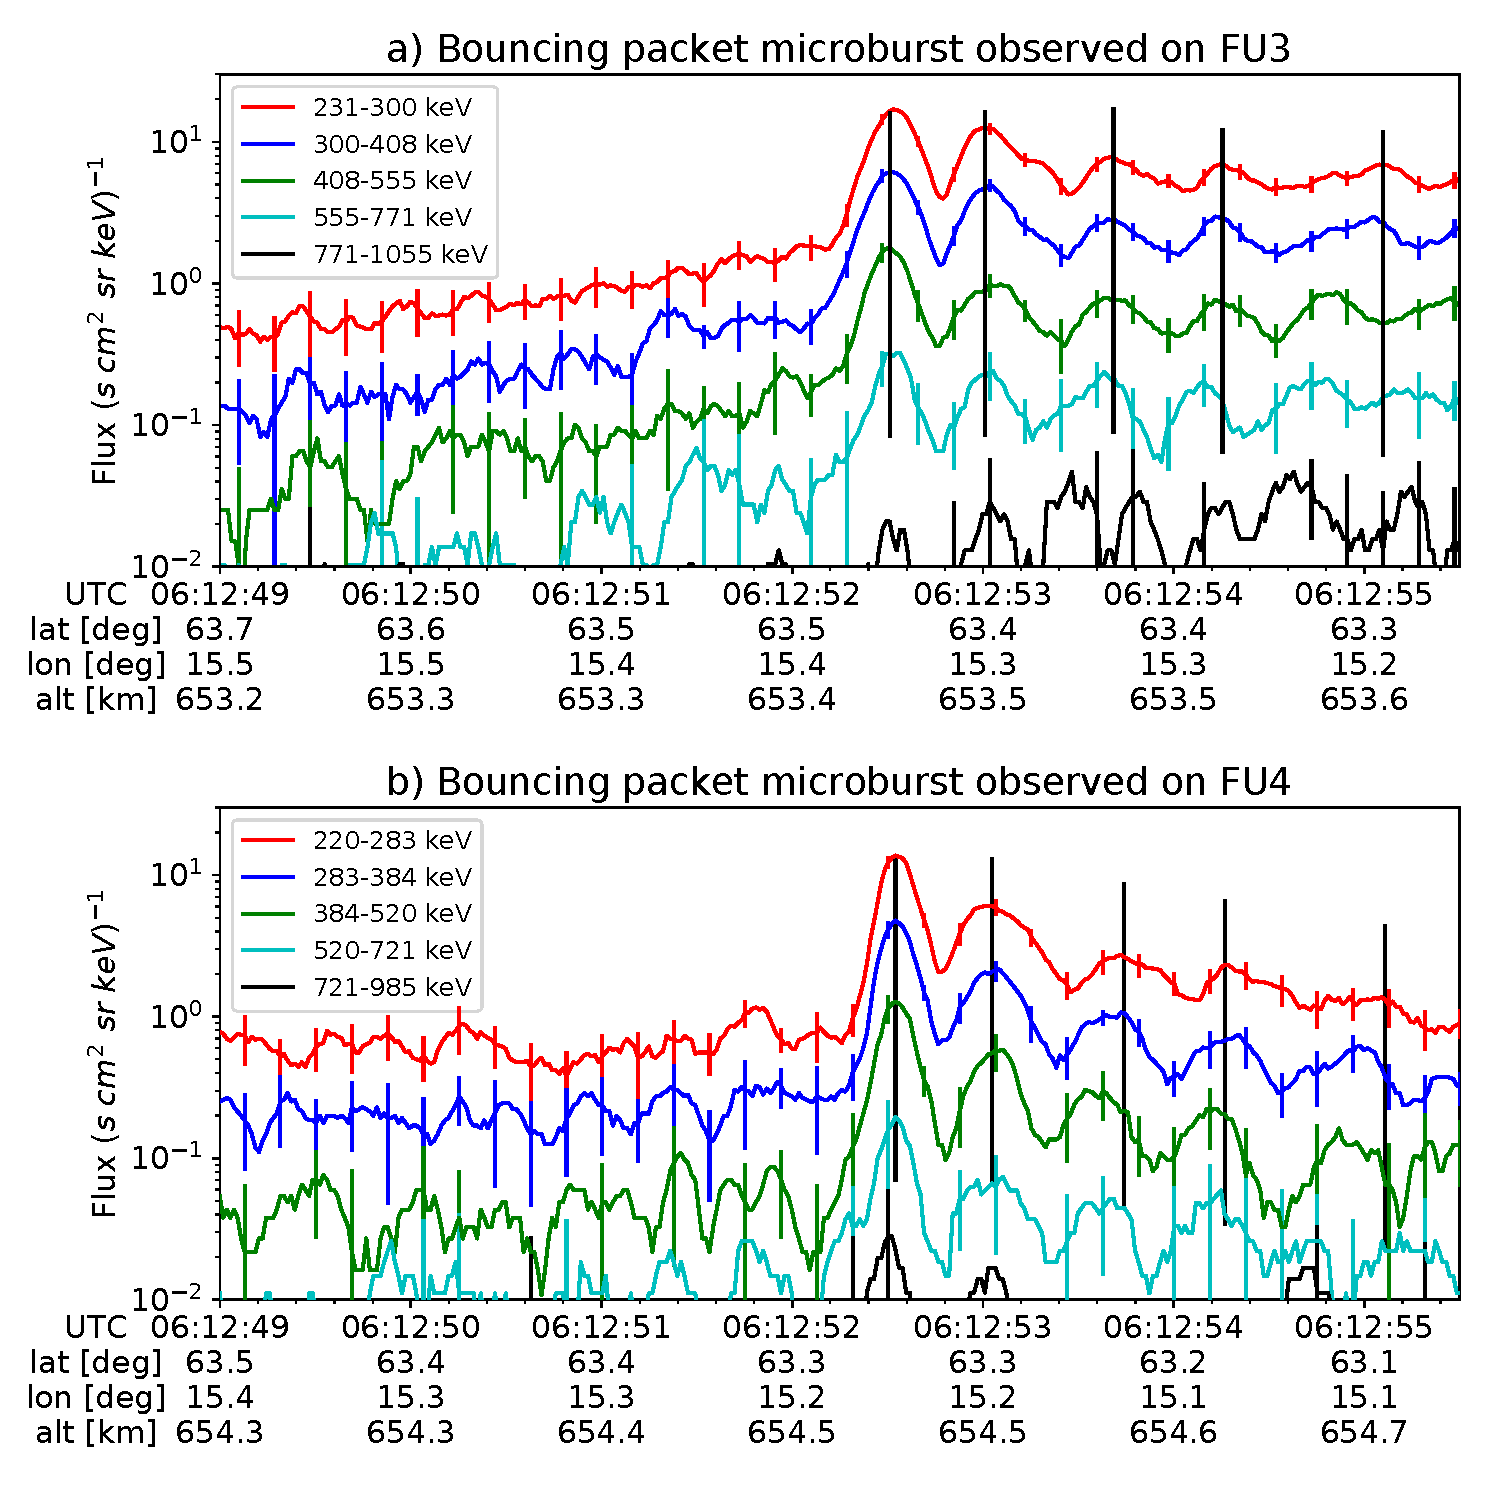
\includegraphics[width=\textwidth]{hires_plot_log_8pt_smooth_pos_v2.pdf}
\caption{HiRes data of the microburst observed at February 2nd, 2015 at 06:12:53 UT, smoothed with a 150 ms rolling average. The subsequent bounces showed some energy dispersion. As discussed in the supporting information, a time correction of -2.28 s was applied to FU3. While the flux from five energy channels is shown, only channels with reasonable counting statistics were used for the spatial scale analysis. Vertical colored bars show the $\sqrt{N}$ error every 10th data point and vertical black bars are lined up with the peaks in the 220-283 keV energy channel to help identify dispersion.}
\label{hires_plot}
\end{figure}

\begin{figure}
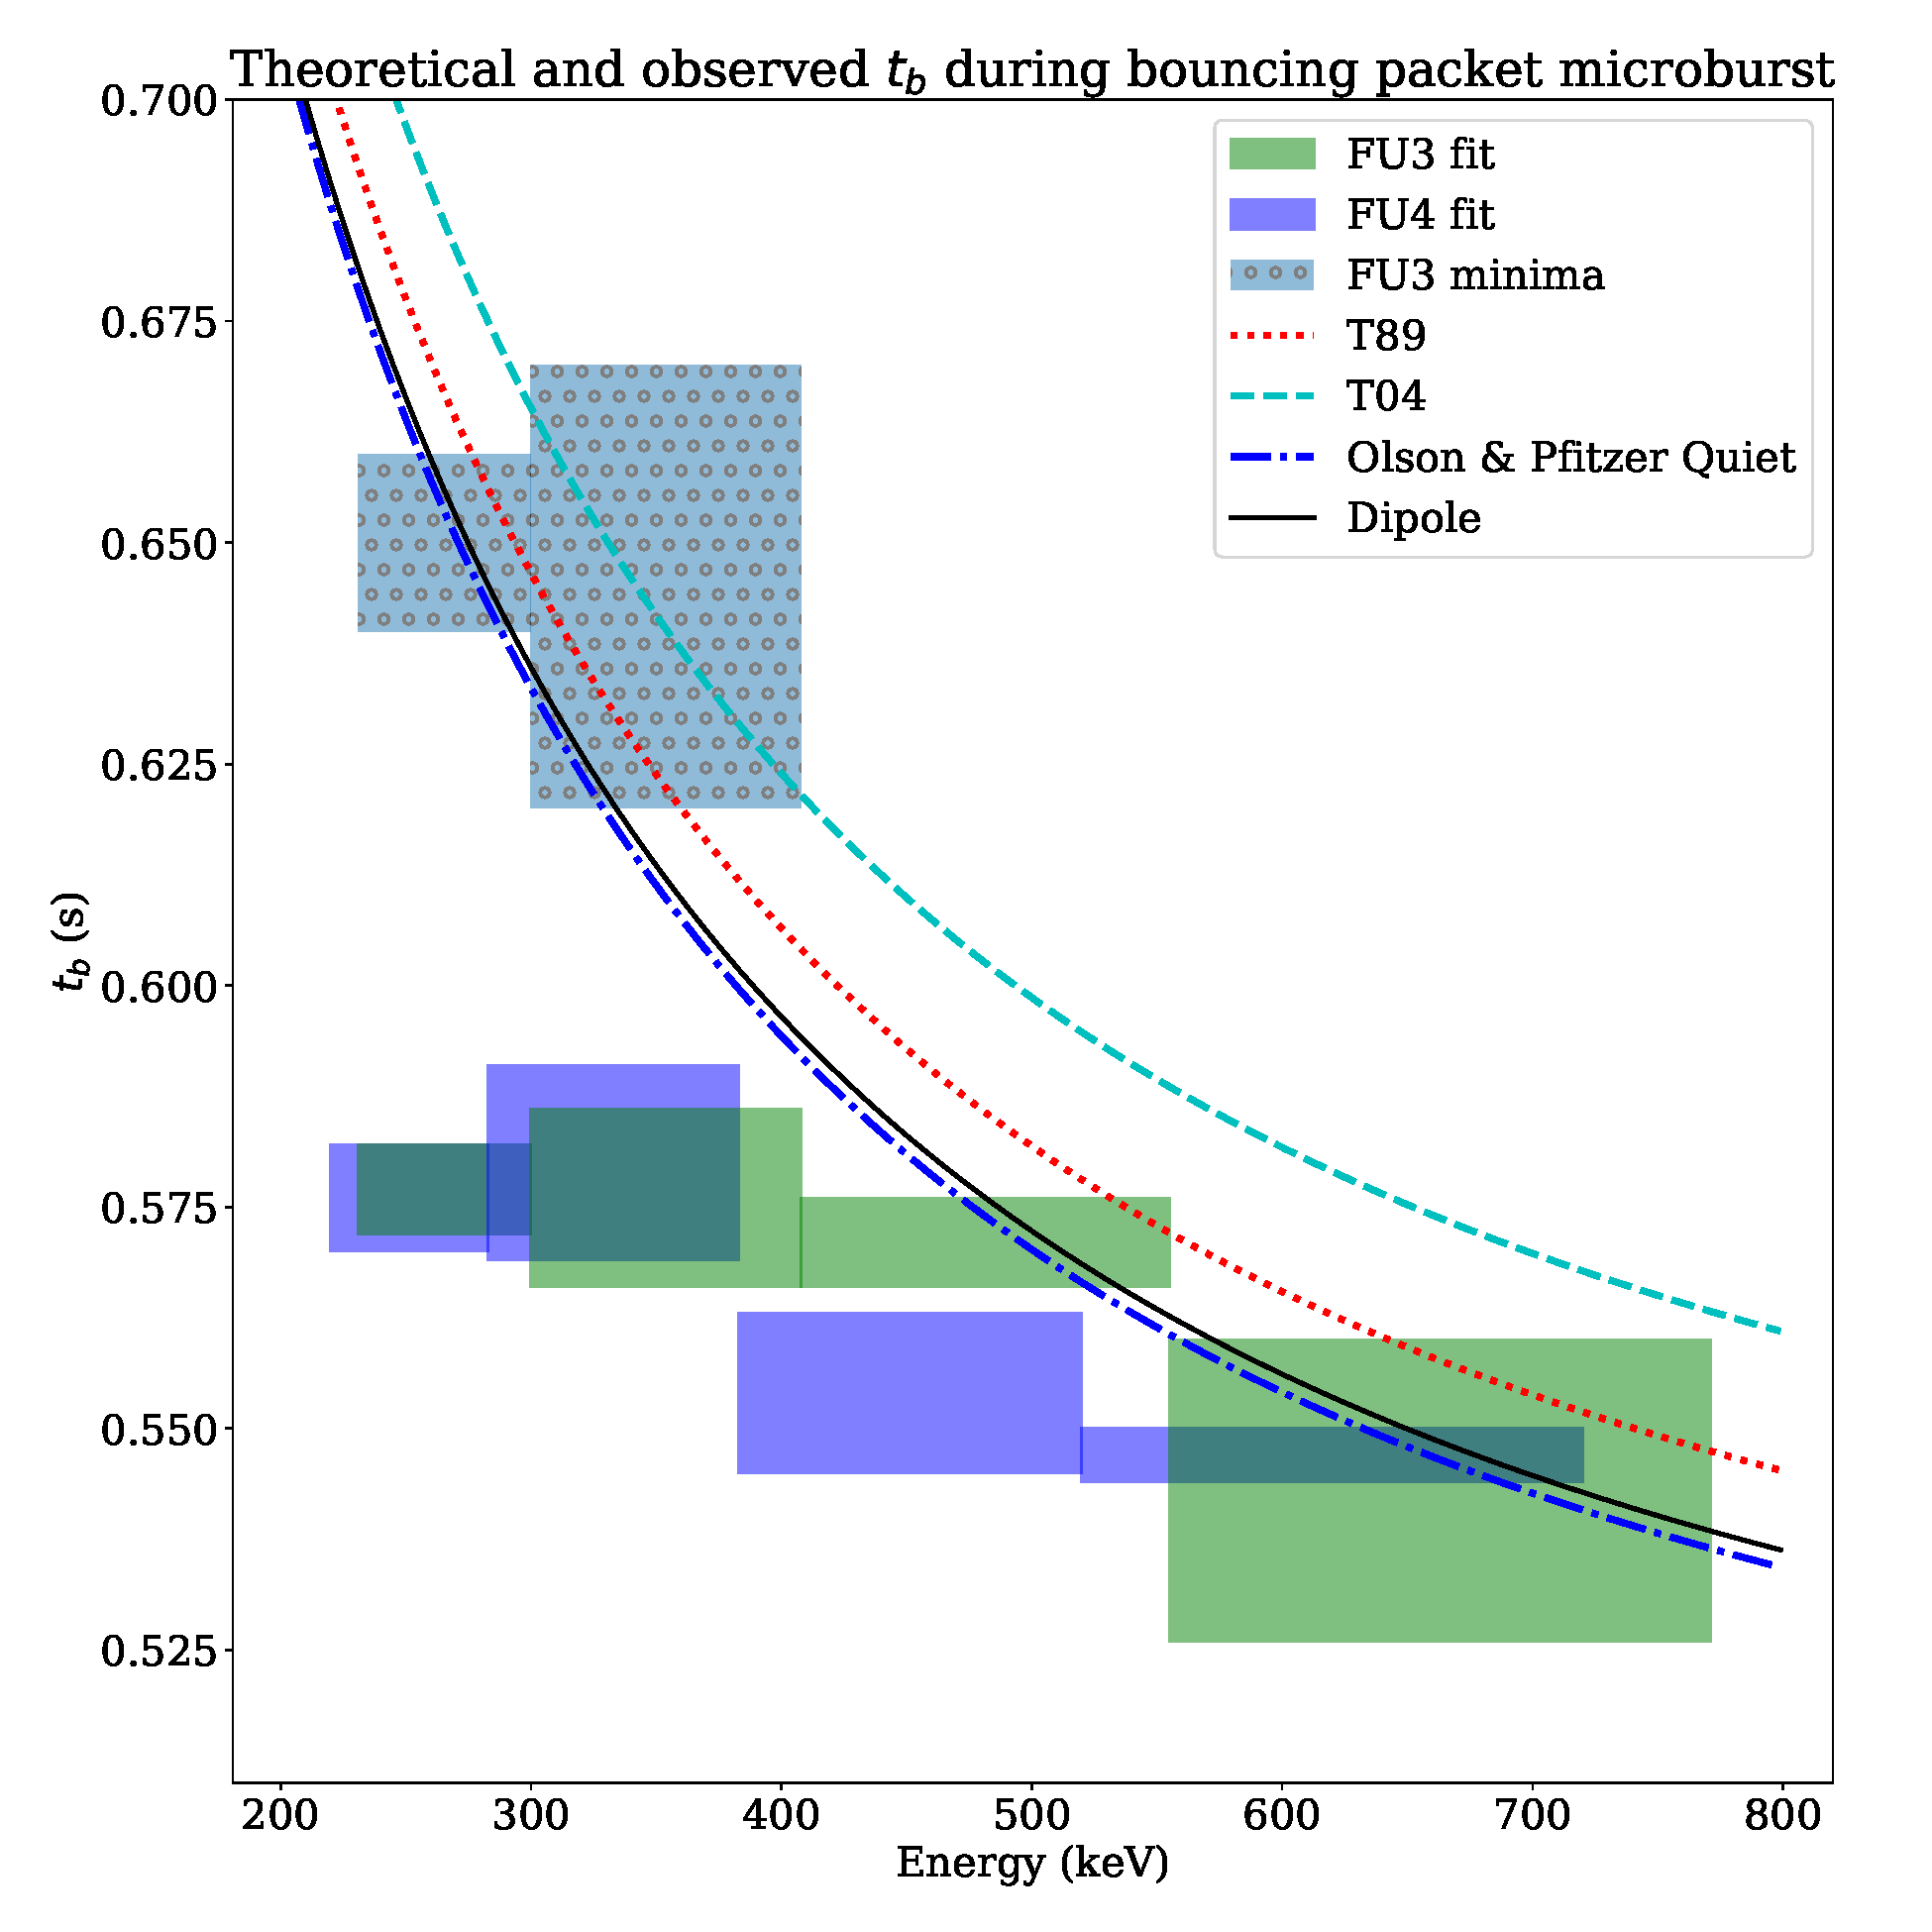
\includegraphics[width=\textwidth]{detrended_bounce_period_boxed_adj.pdf}
\caption{Observed and theoretical $t_b$ for electrons of energies from 200 to 770 keV. The solid black line is $t_b$ in a dipole magnetic field, derived in \citet{Schulz1974}. The red dotted and cyan dashed lines are the $t_b$ derived using the T89, and T04 magnetic field models with IRBEM-Lib. Lastly, the blue dot-dash curve is the $t_b$ derived using the Olson \& Pfitzer Quiet model. The green and purple rectangles represent the observed $t_b$ for FU3 and FU4 using a Gaussian fit, respectively. The blue rectangles represent the observed $t_b$ calculated with the minima between the bounces. The width of the boxes represent the width of those energy channels, and the height represents the uncertainty from the fit.}
\label{tb_plot}
\end{figure}

\begin{figure}
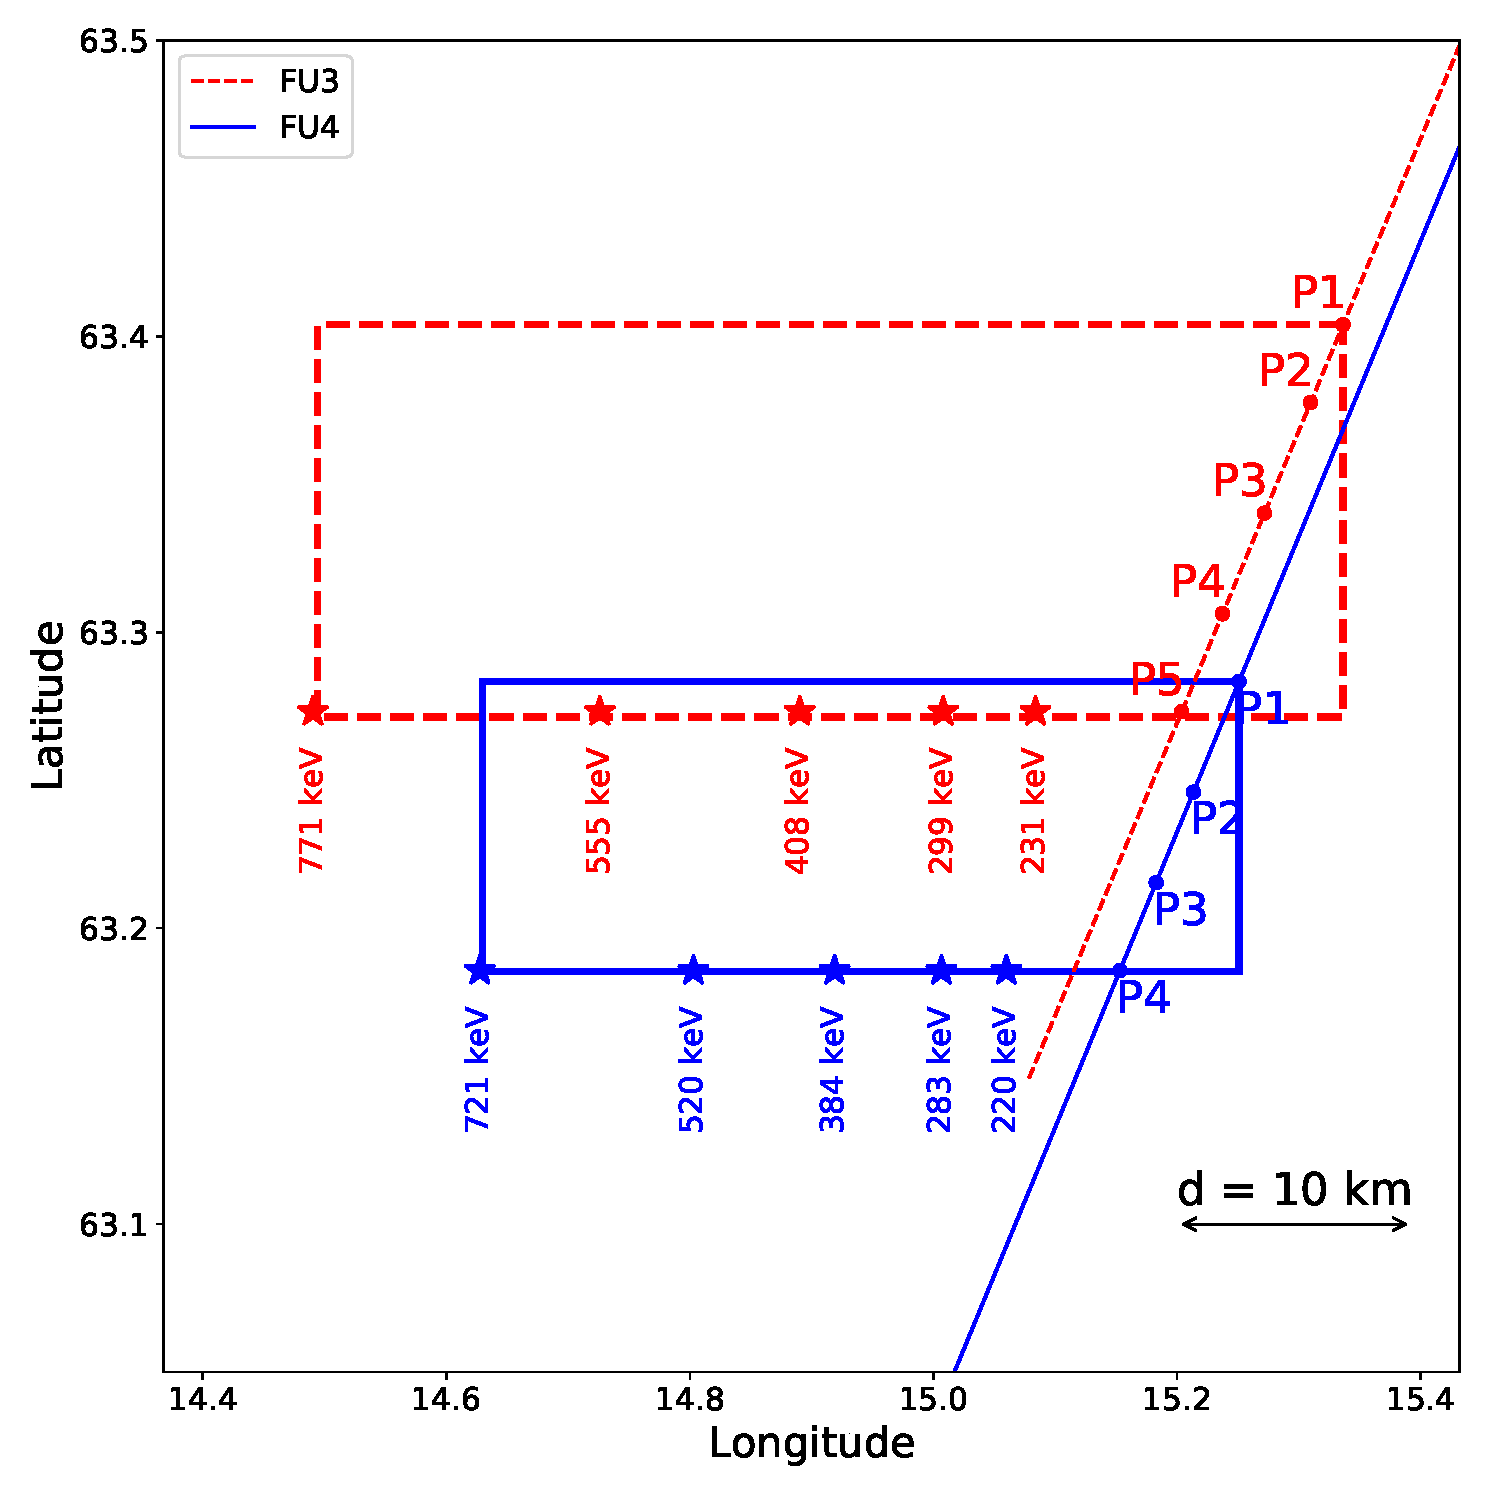
\includegraphics[width=\textwidth]{decay_microburst_distance_corrected_CH4_last_pk_drift_color_3.pdf}
\caption{The topology of the FIREBIRD-II orbit and the multiple bounces of the microburst projected onto latitude and longitude with axis scaled to equal distance. Attributes relating to FU3 shown in red dashed lines, and FU4 with blue solid lines. The spacecraft path is shown with the diagonal lines, starting at the upper right corner. The labels P1-4 for FU4 and P1-5 for FU3 indicate where the spacecraft were when the N$^{th}$ peak was seen in the lowest energy channel in the HiRes data. The stars with the accompanying energy labels represent the locations of the electrons with that energy that started at time of P1, and were seen at the last peak on each spacecraft. The rectangles represent the lower bound of the microburst scale size, assuming that the majority of the electrons were in the upper boundary of energy channel 4.}
\label{map_plot}
\end{figure}

%% ------------------------------------------------------------------------ %%
%% Citations

% Please use ONLY \citet and \citep for reference citations.
% DO NOT use other cite commands (e.g., \cite, \citeyear, \nocite, \citealp, etc.).


%% Example \citet and \citep:
%  ...as shown by \citet{Boug10}, \citet{Buiz07}, \citet{Fra10},
%  \citet{Ghel00}, and \citet{Leit74}. 

%  ...as shown by \citep{Boug10}, \citep{Buiz07}, \citep{Fra10},
%  \citep{Ghel00, Leit74}. 

%  ...has been shown \citep [e.g.,][]{Boug10,Buiz07,Fra10}.

%\bibliography{/home/mike/Dropbox/0_firebird_research/A_presentations/refs}

\begin{thebibliography}{49}
\providecommand{\natexlab}[1]{#1}
\expandafter\ifx\csname urlstyle\endcsname\relax
  \providecommand{\doi}[1]{doi:\discretionary{}{}{}#1}\else
  \providecommand{\doi}{doi:\discretionary{}{}{}\begingroup
  \urlstyle{rm}\Url}\fi

\bibitem[{\textit{Abel and Thorne}(1998)}]{Abel1998_1}
Abel, B., and R.~M. Thorne (1998), Electron scattering loss in earth's inner
  magnetosphere: 1. dominant physical processes, \textit{Journal of Geophysical
  Research: Space Physics}, \textit{103}(A2), 2385--2396.

\bibitem[{\textit{Agapitov et~al.}(2010)\textit{Agapitov, Krasnoselskikh,
  Zaliznyak, Angelopoulos, Le~Contel, and Rolland}}]{Agapitov2010}
Agapitov, O., V.~Krasnoselskikh, Y.~Zaliznyak, V.~Angelopoulos, O.~Le~Contel,
  and G.~Rolland (2010), Chorus source region localization in the earth's outer
  magnetosphere using themis measurements, \textit{Annales Geophysicae},
  \textit{28}(6), 1377--1386, \doi{10.5194/angeo-28-1377-2010}.

\bibitem[{\textit{Agapitov et~al.}(2011)\textit{Agapitov, Krasnoselskikh,
  Dudok~de Wit, Khotyaintsev, Pickett, Santolik, and Rolland}}]{Agapitov2011b}
Agapitov, O., V.~Krasnoselskikh, T.~Dudok~de Wit, Y.~Khotyaintsev, J.~S.
  Pickett, O.~Santolik, and G.~Rolland (2011), Multispacecraft observations of
  chorus emissions as a tool for the plasma density fluctuations' remote
  sensing, \textit{Journal of Geophysical Research: Space Physics},
  \textit{116}(A9), n/a--n/a, \doi{10.1029/2011JA016540}, a09222.

\bibitem[{\textit{Agapitov et~al.}(2017)\textit{Agapitov, Blum, Mozer, Bonnell,
  and Wygant}}]{Agapitov2017a}
Agapitov, O., L.~W. Blum, F.~S. Mozer, J.~W. Bonnell, and J.~Wygant (2017),
  Chorus whistler wave source scales as determined from multipoint van allen
  probe measurements, \textit{Geophysical Research Letters}, pp. n/a--n/a,
  \doi{10.1002/2017GL072701}, 2017GL072701.

\bibitem[{\textit{Anderson et~al.}(2017)\textit{Anderson, Shekhar, Millan,
  Crew, Spence, Klumpar, Blake, O'Brien, and Turner}}]{Anderson2017}
Anderson, B., S.~Shekhar, R.~Millan, A.~Crew, H.~Spence, D.~Klumpar, J.~Blake,
  T.~O'Brien, and D.~Turner (2017), Spatial scale and duration of one
  microburst region on 13 august 2015, \textit{Journal of Geophysical Research:
  Space Physics}.

\bibitem[{\textit{Anderson and Milton}(1964)}]{Anderson1964}
Anderson, K.~A., and D.~W. Milton (1964), Balloon observations of x rays in the
  auroral zone: 3. high time resolution studies, \textit{Journal of Geophysical
  Research}, \textit{69}(21), 4457--4479, \doi{10.1029/JZ069i021p04457}.

\bibitem[{\textit{Blake et~al.}(1996)\textit{Blake, Looper, Baker, Nakamura,
  Klecker, and Hovestadt}}]{Blake1996}
Blake, J., M.~Looper, D.~Baker, R.~Nakamura, B.~Klecker, and D.~Hovestadt
  (1996), New high temporal and spatial resolution measurements by sampex of
  the precipitation of relativistic electrons, \textit{Advances in Space
  Research}, \textit{18}(8), 171 -- 186,
  \doi{http://dx.doi.org/10.1016/0273-1177(95)00969-8}.

\bibitem[{\textit{Blum et~al.}(2015)\textit{Blum, Li, and Denton}}]{Blum2015}
Blum, L., X.~Li, and M.~Denton (2015), Rapid mev electron precipitation as
  observed by sampex/hilt during high-speed stream-driven storms,
  \textit{Journal of Geophysical Research: Space Physics}, \textit{120}(5),
  3783--3794, \doi{10.1002/2014JA020633}, 2014JA020633.

\bibitem[{\textit{Boscher et~al.}(2012)\textit{Boscher, Bourdarie, O'Brien,
  Guild, and Shumko}}]{irbem}
Boscher, D., S.~Bourdarie, P.~O'Brien, T.~Guild, and M.~Shumko (2012),
  Irbem-lib library.

\bibitem[{\textit{Breneman et~al.}(2017)\textit{Breneman, Crew, Sample,
  Klumpar, Johnson, Agapitov, Shumko, Turner, Santolik, Wygant
  et~al.}}]{Breneman2017}
Breneman, A., A.~Crew, J.~Sample, D.~Klumpar, A.~Johnson, O.~Agapitov,
  M.~Shumko, D.~Turner, O.~Santolik, J.~Wygant, et~al. (2017), Observations
  directly linking relativistic electron microbursts to whistler mode chorus:
  Van allen probes and firebird ii, \textit{Geophysical Research Letters}.

\bibitem[{\textit{Comess et~al.}(2013)\textit{Comess, Smith, Selesnick, Millan,
  and Sample}}]{Comess2013}
Comess, M., D.~Smith, R.~Selesnick, R.~Millan, and J.~Sample (2013), Duskside
  relativistic electron precipitation as measured by sampex: A statistical
  survey, \textit{Journal of Geophysical Research: Space Physics},
  \textit{118}(8), 5050--5058, \doi{10.1002/jgra.50481}.

\bibitem[{\textit{Crew et~al.}(2016)\textit{Crew, Spence, Blake, Klumpar,
  Larsen, O'Brien, Driscoll, Handley, Legere, Longworth, Mashburn, Mosleh,
  Ryhajlo, Smith, Springer, and Widholm}}]{Crew2016}
Crew, A.~B., H.~E. Spence, J.~B. Blake, D.~M. Klumpar, B.~A. Larsen, T.~P.
  O'Brien, S.~Driscoll, M.~Handley, J.~Legere, S.~Longworth, K.~Mashburn,
  E.~Mosleh, N.~Ryhajlo, S.~Smith, L.~Springer, and M.~Widholm (2016), First
  multipoint in situ observations of electron microbursts: Initial results from
  the nsf firebird ii mission, \textit{Journal of Geophysical Research: Space
  Physics}, \textit{121}(6), 5272--5283, \doi{10.1002/2016JA022485},
  2016JA022485.

\bibitem[{\textit{Datta et~al.}(1997)\textit{Datta, Skoug, McCarthy, and
  Parks}}]{Datta1997}
Datta, S., R.~Skoug, M.~McCarthy, and G.~Parks (1997), Modeling of microburst
  electron precipitation using pitch angle diffusion theory, \textit{Journal of
  Geophysical Research: Space Physics}, \textit{102}(A8), 17,325--17,333.

\bibitem[{\textit{Dietrich et~al.}(2010)\textit{Dietrich, Rodger, Clilverd,
  Bortnik, and Raita}}]{Dietrich2010}
Dietrich, S., C.~J. Rodger, M.~A. Clilverd, J.~Bortnik, and T.~Raita (2010),
  Relativistic microburst storm characteristics: Combined satellite and
  ground-based observations, \textit{Journal of Geophysical Research: Space
  Physics}, \textit{115}(A12).

\bibitem[{\textit{Fang et~al.}(2010)\textit{Fang, Randall, Lummerzheim, Wang,
  Lu, Solomon, and Frahm}}]{Fang2010}
Fang, X., C.~E. Randall, D.~Lummerzheim, W.~Wang, G.~Lu, S.~C. Solomon, and
  R.~A. Frahm (2010), Parameterization of monoenergetic electron impact
  ionization, \textit{Geophysical Research Letters}, \textit{37}(22).

\bibitem[{\textit{Gurnett et~al.}(1979)\textit{Gurnett, Anderson, Scarf,
  Fredricks, and Smith}}]{Gurnett1979}
Gurnett, D., R.~Anderson, F.~Scarf, R.~Fredricks, and E.~Smith (1979), Initial
  results from the isee-1 and-2 plasma wave investigation, \textit{Space
  Science Reviews}, \textit{23}(1), 103--122.

\bibitem[{\textit{Horne and Thorne}(2003)}]{Horne2003}
Horne, R.~B., and R.~M. Thorne (2003), Relativistic electron acceleration and
  precipitation during resonant interactions with whistler-mode chorus,
  \textit{Geophysical Research Letters}, \textit{30}(10), n/a--n/a,
  \doi{10.1029/2003GL016973}, 1527.

\bibitem[{\textit{Kletzing et~al.}(2013)\textit{Kletzing, Kurth, Acuna,
  MacDowall, Torbert, Averkamp, Bodet, Bounds, Chutter, Connerney
  et~al.}}]{Kletzing2013}
Kletzing, C., W.~Kurth, M.~Acuna, R.~MacDowall, R.~Torbert, T.~Averkamp,
  D.~Bodet, S.~Bounds, M.~Chutter, J.~Connerney, et~al. (2013), The electric
  and magnetic field instrument suite and integrated science (emfisis) on rbsp,
  \textit{Space Science Reviews}, \textit{179}(1-4), 127--181.

\bibitem[{\textit{Klumpar et~al.}(2015)\textit{Klumpar, Springer, Mosleh,
  Mashburn, Berardinelli, Gunderson, Handly, Ryhajlo, Spence, Smith, Legere,
  Widholm, Longworth, Crew, Larsen, Blake, and Walmsley}}]{Klumpar2015}
Klumpar, D., L.~Springer, E.~Mosleh, K.~Mashburn, S.~Berardinelli,
  A.~Gunderson, M.~Handly, N.~Ryhajlo, H.~Spence, S.~Smith, J.~Legere,
  M.~Widholm, S.~Longworth, A.~Crew, B.~Larsen, J.~Blake, and N.~Walmsley
  (2015), Flight system technologies enabling the twin-cubesat firebird-ii
  scientific mission.

\bibitem[{\textit{Lee et~al.}(2005)\textit{Lee, Parks, Min, Kim, Park, Hwang,
  McCarthy, Lee, Ryu, Lim, Sim, Lee, Kang, and Park}}]{Lee2005}
Lee, J.-J., G.~K. Parks, K.~W. Min, H.~J. Kim, J.~Park, J.~Hwang, M.~P.
  McCarthy, E.~Lee, K.~S. Ryu, J.~T. Lim, E.~S. Sim, H.~W. Lee, K.~I. Kang, and
  H.~Y. Park (2005), Energy spectra of 170-360 kev electron microbursts
  measured by the korean stsat-1, \textit{Geophysical Research Letters},
  \textit{32}(13), \doi{10.1029/2005GL022996}, l13106.

\bibitem[{\textit{Lee et~al.}(2012)\textit{Lee, Parks, Lee, Tsurutani, Hwang,
  Cho, Kim, Park, Min, and McCarthy}}]{Lee2012}
Lee, J.~J., G.~K. Parks, E.~Lee, B.~T. Tsurutani, J.~Hwang, K.~S. Cho, K.-H.
  Kim, Y.~D. Park, K.~W. Min, and M.~P. McCarthy (2012), Anisotropic pitch
  angle distribution of ~100 kev microburst electrons in the loss cone:
  measurements from stsat-1, \textit{Annales Geophysicae}, \textit{30}(11),
  1567--1573, \doi{10.5194/angeo-30-1567-2012}.

\bibitem[{\textit{Li et~al.}(2009)\textit{Li, Thorne, Angelopoulos, Bortnik,
  Cully, Ni, LeContel, Roux, Auster, and Magnes}}]{Li2009}
Li, W., R.~M. Thorne, V.~Angelopoulos, J.~Bortnik, C.~M. Cully, B.~Ni,
  O.~LeContel, A.~Roux, U.~Auster, and W.~Magnes (2009), Global distribution of
  whistler-mode chorus waves observed on the themis spacecraft,
  \textit{Geophysical Research Letters}, \textit{36}(9), n/a--n/a,
  \doi{10.1029/2009GL037595}, l09104.

\bibitem[{\textit{Lorentzen et~al.}(2001{\natexlab{a}})\textit{Lorentzen,
  Blake, Inan, and Bortnik}}]{Lorentzen2001a}
Lorentzen, K.~R., J.~B. Blake, U.~S. Inan, and J.~Bortnik (2001{\natexlab{a}}),
  Observations of relativistic electron microbursts in association with vlf
  chorus, \textit{Journal of Geophysical Research: Space Physics},
  \textit{106}(A4), 6017--6027, \doi{10.1029/2000JA003018}.

\bibitem[{\textit{Lorentzen et~al.}(2001{\natexlab{b}})\textit{Lorentzen,
  Looper, and Blake}}]{Lorentzen2001b}
Lorentzen, K.~R., M.~D. Looper, and J.~B. Blake (2001{\natexlab{b}}),
  Relativistic electron microbursts during the gem storms, \textit{Geophysical
  Research Letters}, \textit{28}(13), 2573--2576, \doi{10.1029/2001GL012926}.

\bibitem[{\textit{Mauk et~al.}(2013)\textit{Mauk, Fox, Kanekal, Kessel, Sibeck,
  and Ukhorskiy}}]{Mauk2013}
Mauk, B., N.~J. Fox, S.~Kanekal, R.~Kessel, D.~Sibeck, and A.~Ukhorskiy (2013),
  Science objectives and rationale for the radiation belt storm probes mission,
  \textit{Space Science Reviews}, \textit{179}(1-4), 3--27.

\bibitem[{\textit{Meredith et~al.}(2002)\textit{Meredith, Horne, Summers,
  Thorne, Iles, Heynderickx, and Anderson}}]{Meredith2002}
Meredith, N., R.~Horne, D.~Summers, R.~Thorne, R.~Iles, D.~Heynderickx, and
  R.~Anderson (2002), Evidence for acceleration of outer zone electrons to
  relativistic energies by whistler mode chorus, in \textit{Annales
  Geophysicae}, vol.~20, pp. 967--979.

\bibitem[{\textit{Millan and Thorne}(2007)}]{Millan2007}
Millan, R., and R.~Thorne (2007), Review of radiation belt relativistic
  electron losses, \textit{Journal of Atmospheric and Solar-Terrestrial
  Physics}, \textit{69}(3), 362 -- 377,
  \doi{http://dx.doi.org/10.1016/j.jastp.2006.06.019}, global Aspects of
  Magnetosphere-Ionosphere CouplingGlobal Aspects of Magnetosphere-Ionosphere
  Coupling.

\bibitem[{\textit{Millan et~al.}(2002)\textit{Millan, Lin, Smith, Lorentzen,
  and McCarthy}}]{Millan2002}
Millan, R.~M., R.~Lin, D.~Smith, K.~Lorentzen, and M.~McCarthy (2002), X-ray
  observations of mev electron precipitation with a balloon-borne germanium
  spectrometer, \textit{Geophysical research letters}, \textit{29}(24).

\bibitem[{\textit{Mozer et~al.}(2018)\textit{Mozer, Agapitov, Blake, and
  Vasko}}]{Mozer2018}
Mozer, F.~S., O.~V. Agapitov, J.~B. Blake, and I.~Y. Vasko (2018), Simultaneous
  observations of lower band chorus emissions at the equator and microburst
  precipitating electrons in the ionosphere, \textit{Geophysical Research
  Letters}, pp. n/a--n/a, \doi{10.1002/2017GL076120}, 2017GL076120.

\bibitem[{\textit{Nakamura et~al.}(1995)\textit{Nakamura, Baker, Blake,
  Kanekal, Klecker, and Hovestadt}}]{Nakamura1995}
Nakamura, R., D.~N. Baker, J.~B. Blake, S.~Kanekal, B.~Klecker, and
  D.~Hovestadt (1995), Relativistic electron precipitation enhancements near
  the outer edge of the radiation belt, \textit{Geophysical Research Letters},
  \textit{22}(9), 1129--1132, \doi{10.1029/95GL00378}.

\bibitem[{\textit{Nakamura et~al.}(2000)\textit{Nakamura, Isowa, Kamide, Baker,
  Blake, and Looper}}]{Nakamura2000}
Nakamura, R., M.~Isowa, Y.~Kamide, D.~Baker, J.~Blake, and M.~Looper (2000),
  Observations of relativistic electron microbursts in association with vlf
  chorus, \textit{J. Geophys. Res}, \textit{105}, 15,875--15,885.

\bibitem[{\textit{O'Brien et~al.}(2003)\textit{O'Brien, Lorentzen, Mann,
  Meredith, Blake, Fennell, Looper, Milling, and Anderson}}]{O'Brien2003}
O'Brien, T.~P., K.~R. Lorentzen, I.~R. Mann, N.~P. Meredith, J.~B. Blake, J.~F.
  Fennell, M.~D. Looper, D.~K. Milling, and R.~R. Anderson (2003), Energization
  of relativistic electrons in the presence of ulf power and mev microbursts:
  Evidence for dual ulf and vlf acceleration, \textit{Journal of Geophysical
  Research: Space Physics}, \textit{108}(A8), n/a--n/a,
  \doi{10.1029/2002JA009784}, 1329.

\bibitem[{\textit{O'Brien et~al.}(2004)\textit{O'Brien, Looper, and
  Blake}}]{O'Brien2004}
O'Brien, T.~P., M.~D. Looper, and J.~B. Blake (2004), Quantification of
  relativistic electron microburst losses during the gem storms,
  \textit{Geophysical Research Letters}, \textit{31}(4), n/a--n/a,
  \doi{10.1029/2003GL018621}, l04802.

\bibitem[{\textit{Olson and Pfitzer}(1982)}]{Olson1982}
Olson, W.~P., and K.~A. Pfitzer (1982), A dynamic model of the magnetospheric
  magnetic and electric fields for july 29, 1977, \textit{Journal of
  Geophysical Research: Space Physics}, \textit{87}(A8), 5943--5948,
  \doi{10.1029/JA087iA08p05943}.

\bibitem[{\textit{Parks}(2003)}]{Parks2003}
Parks, G. (2003), \textit{Physics Of Space Plasmas: An Introduction, Second
  Edition}, Westview Press.

\bibitem[{\textit{Parks}(1967)}]{Parks1967}
Parks, G.~K. (1967), Spatial characteristics of auroral-zone x-ray microbursts,
  \textit{Journal of Geophysical Research}, \textit{72}(1), 215--226.

\bibitem[{\textit{Santolik et~al.}(2003)\textit{Santolik, Gurnett, Pickett,
  Parrot, and Cornilleau-Wehrlin}}]{Santolik2003}
Santolik, O., D.~Gurnett, J.~Pickett, M.~Parrot, and N.~Cornilleau-Wehrlin
  (2003), Spatio-temporal structure of storm-time chorus, \textit{Journal of
  Geophysical Research: Space Physics}, \textit{108}(A7).

\bibitem[{\textit{Schulz and Lanzerotti}(1974)}]{Schulz1974}
Schulz, M., and L.~J. Lanzerotti (1974), \textit{Particle Diffusion in the
  Radiation Belts}, Springer.

\bibitem[{\textit{Selesnick et~al.}(2003)\textit{Selesnick, Blake, and
  Mewaldt}}]{Selesnick2003}
Selesnick, R.~S., J.~B. Blake, and R.~A. Mewaldt (2003), Atmospheric losses of
  radiation belt electrons, \textit{Journal of Geophysical Research: Space
  Physics}, \textit{108}(A12), \doi{10.1029/2003JA010160}, 1468.

\bibitem[{\textit{Shprits and Thorne}(2004)}]{Shprits2004}
Shprits, Y.~Y., and R.~M. Thorne (2004), Time dependent radial diffusion
  modeling of relativistic electrons with realistic loss rates,
  \textit{Geophysical Research Letters}, \textit{31}(8), n/a--n/a,
  \doi{10.1029/2004GL019591}, l08805.

\bibitem[{\textit{Shprits et~al.}(2007)\textit{Shprits, Meredith, and
  Thorne}}]{Shprits2007}
Shprits, Y.~Y., N.~P. Meredith, and R.~M. Thorne (2007), Parameterization of
  radiation belt electron loss timescales due to interactions with chorus
  waves, \textit{Geophysical Research Letters}, \textit{34}(11), n/a--n/a,
  \doi{10.1029/2006GL029050}, l11110.

\bibitem[{\textit{Spence et~al.}(2012)\textit{Spence, Blake, Crew, Driscoll,
  Klumpar, Larsen, Legere, Longworth, Mosleh, O'Brien, Smith, Springer, and
  Widholm}}]{Spence2012}
Spence, H.~E., J.~B. Blake, A.~B. Crew, S.~Driscoll, D.~M. Klumpar, B.~A.
  Larsen, J.~Legere, S.~Longworth, E.~Mosleh, T.~P. O'Brien, S.~Smith,
  L.~Springer, and M.~Widholm (2012), Focusing on size and energy dependence of
  electron microbursts from the van allen radiation belts, \textit{Space
  Weather}, \textit{10}(11), \doi{10.1029/2012SW000869}.

\bibitem[{\textit{Summers et~al.}(1998)\textit{Summers, Thorne, and
  Xiao}}]{Summers1998}
Summers, D., R.~M. Thorne, and F.~Xiao (1998), Relativistic theory of
  wave-particle resonant diffusion with application to electron acceleration in
  the magnetosphere, \textit{Journal of Geophysical Research: Space Physics},
  \textit{103}(A9), 20,487--20,500.

\bibitem[{\textit{Thorne}(2010)}]{Thorne2010}
Thorne, R.~M. (2010), Radiation belt dynamics: The importance of wave-particle
  interactions, \textit{Geophysical Research Letters}, \textit{37}(22),
  \doi{10.1029/2010GL044990}, l22107.

\bibitem[{\textit{Thorne et~al.}(2005)\textit{Thorne, O'Brien, Shprits,
  Summers, and Horne}}]{Thorne2005}
Thorne, R.~M., T.~P. O'Brien, Y.~Y. Shprits, D.~Summers, and R.~B. Horne
  (2005), Timescale for mev electron microburst loss during geomagnetic storms,
  \textit{Journal of Geophysical Research: Space Physics}, \textit{110}(A9),
  n/a--n/a, \doi{10.1029/2004JA010882}, a09202.

\bibitem[{\textit{Tsyganenko}(1989)}]{Tsyganenko1989}
Tsyganenko, N. (1989), A solution of the chapman-ferraro problem for an
  ellipsoidal magnetopause, \textit{Planetary and Space Science},
  \textit{37}(9), 1037 -- 1046,
  \doi{http://dx.doi.org/10.1016/0032-0633(89)90076-7}.

\bibitem[{\textit{Tsyganenko and Sitnov}(2005)}]{Tsyganenko2005}
Tsyganenko, N.~A., and M.~I. Sitnov (2005), Modeling the dynamics of the inner
  magnetosphere during strong geomagnetic storms, \textit{Journal of
  Geophysical Research: Space Physics}, \textit{110}(A3), n/a--n/a,
  \doi{10.1029/2004JA010798}, a03208.

\bibitem[{\textit{Ukhorskiy et~al.}(2006)\textit{Ukhorskiy, Anderson, Brandt,
  and Tsyganenko}}]{Ukhorskiy2006}
Ukhorskiy, A.~Y., B.~J. Anderson, P.~C. Brandt, and N.~A. Tsyganenko (2006),
  Storm time evolution of the outer radiation belt: Transport and losses,
  \textit{Journal of Geophysical Research: Space Physics}, \textit{111}(A11),
  n/a--n/a, \doi{10.1029/2006JA011690}, a11S03.

\bibitem[{\textit{Woodger et~al.}(2015)\textit{Woodger, Halford, Millan,
  McCarthy, Smith, Bowers, Sample, Anderson, and Liang}}]{Woodger2015}
Woodger, L., A.~Halford, R.~Millan, M.~McCarthy, D.~Smith, G.~Bowers,
  J.~Sample, B.~Anderson, and X.~Liang (2015), A summary of the barrel
  campaigns: Technique for studying electron precipitation, \textit{Journal of
  Geophysical Research: Space Physics}, \textit{120}(6), 4922--4935.

\end{thebibliography}

%%  REFERENCE LIST AND TEXT CITATIONS
%
% Either type in your references using
%
% \begin{thebibliography}{}
% \bibitem[{\textit{Kobayashi et~al.}}(2003)]{R2013} Kobayashi, T.,
% Tran, A.~H., Nishijo, H., Ono, T., and Matsumoto, G.  (2003).
% Contribution of hippocampal place cell activity to learning and
% formation of goal-directed navigation in rats. \textit{Neuroscience}
% 117, 1025--1035.
%
% \bibitem{}
% Text
% \end{thebibliography}
%
%%%%%%%%%%%%%%%%%%%%%%%%%%%%%%%%%%%%%%%%%%%%%%%
% Or, to use BibTeX:
%
% Follow these steps
%
% 1. Type in \bibliography{<name of your .bib file>} 
%    Run LaTeX on your LaTeX file.
%
% 2. Run BiBTeX on your LaTeX file.
%
% 3. Open the new .bbl file containing the reference list and
%   copy all the contents into your LaTeX file here.
%
% 4. Run LaTeX on your new file which will produce the citations.
%
% AGU does not want a .bib or a .bbl file. Please copy in the contents of your .bbl file here.


%% After you run BibTeX, Copy in the contents of the .bbl file here:
%\begin{thebibliography}{35}
%\end{thebibliography}

%%%%%%%%%%%%%%%%%%%%%%%%%%%%%%%%%%%%%%%%%%%%%%%%%%%%%%%%%%%%%%%%%%%%%
% Track Changes:
% To add words, \added{<word added>}
% To delete words, \deleted{<word deleted>}
% To replace words, \replace{<word to be replaced>}{<replacement word>}
% To explain why change was made: \explain{<explanation>} This will put
% a comment into the right margin.

%%%%%%%%%%%%%%%%%%%%%%%%%%%%%%%%%%%%%%%%%%%%%%%%%%%%%%%%%%%%%%%%%%%%%
% At the end of the document, use \listofchanges, which will list the
% changes and the page and line number where the change was made.

% When final version, \listofchanges will not produce anything,
% \added{<word or words>} word will be printed, \deleted{<word or words} will take away the word,
% \replaced{<delete this word>}{<replace with this word>} will print only the replacement word.
%  In the final version, \explain will not print anything.
%%%%%%%%%%%%%%%%%%%%%%%%%%%%%%%%%%%%%%%%%%%%%%%%%%%%%%%%%%%%%%%%%%%%%

%%%
%\listofchanges
%%%

\end{document}

%%%%%%%%%%%%%%%%%%%%%%%%%%%%%%%%%%%%%
%% Supporting Information
%% (Optional) See AGUSuppInfoSamp.tex/pdf for requirements 
%% for Supporting Information.
%%%%%%%%%%%%%%%%%%%%%%%%%%%%%%%%%%%%%



%%%%%%%%%%%%%%%%%%%%%%%%%%%%%%%%%%%%%%%%%%%%%%%%%%%%%%%%%%%%%%%

More Information and Advice:

%% ------------------------------------------------------------------------ %%
%
%  SECTION HEADS
%
%% ------------------------------------------------------------------------ %%

% Capitalize the first letter of each word (except for
% prepositions, conjunctions, and articles that are
% three or fewer letters).

% AGU follows standard outline style; therefore, there cannot be a section 1 without
% a section 2, or a section 2.3.1 without a section 2.3.2.
% Please make sure your section numbers are balanced.
% ---------------
% Level 1 head
%
% Use the \section{} command to identify level 1 heads;
% type the appropriate head wording between the curly
% brackets, as shown below.
%
%An example:
%\section{Level 1 Head: Introduction}
%
% ---------------
% Level 2 head
%
% Use the \subsection{} command to identify level 2 heads.
%An example:
%\subsection{Level 2 Head}
%
% ---------------
% Level 3 head
%
% Use the \subsubsection{} command to identify level 3 heads
%An example:
%\subsubsection{Level 3 Head}
%
%---------------
% Level 4 head
%
% Use the \subsubsubsection{} command to identify level 3 heads
% An example:
%\subsubsubsection{Level 4 Head} An example.
%
%% ------------------------------------------------------------------------ %%
%
%  IN-TEXT LISTS
%
%% ------------------------------------------------------------------------ %%
%
% Do not use bulleted lists; enumerated lists are okay.
% \begin{enumerate}
% \item
% \item
% \item
% \end{enumerate}
%
%% ------------------------------------------------------------------------ %%
%
%  EQUATIONS
%
%% ------------------------------------------------------------------------ %%

% Single-line equations are centered.
% Equation arrays will appear left-aligned.

Math coded inside display math mode \[ ...\]
 will not be numbered, e.g.,:
 \[ x^2=y^2 + z^2\]

 Math coded inside \begin{equation} and \end{equation} will
 be automatically numbered, e.g.,:
 \begin{equation}
 x^2=y^2 + z^2
 \end{equation}


% To create multiline equations, use the
% \begin{eqnarray} and \end{eqnarray} environment
% as demonstrated below.
\begin{eqnarray}
  x_{1} & = & (x - x_{0}) \cos \Theta \nonumber \\
        && + (y - y_{0}) \sin \Theta  \nonumber \\
  y_{1} & = & -(x - x_{0}) \sin \Theta \nonumber \\
        && + (y - y_{0}) \cos \Theta.
\end{eqnarray}

%If you don't want an equation number, use the star form:
%\begin{eqnarray*}...\end{eqnarray*}

% Break each line at a sign of operation
% (+, -, etc.) if possible, with the sign of operation
% on the new line.

% Indent second and subsequent lines to align with
% the first character following the equal sign on the
% first line.

% Use an \hspace{} command to insert horizontal space
% into your equation if necessary. Place an appropriate
% unit of measure between the curly braces, e.g.
% \hspace{1in}; you may have to experiment to achieve
% the correct amount of space.


%% ------------------------------------------------------------------------ %%
%
%  EQUATION NUMBERING: COUNTER
%
%% ------------------------------------------------------------------------ %%

% You may change equation numbering by resetting
% the equation counter or by explicitly numbering
% an equation.

% To explicitly number an equation, type \eqnum{}
% (with the desired number between the brackets)
% after the \begin{equation} or \begin{eqnarray}
% command.  The \eqnum{} command will affect only
% the equation it appears with; LaTeX will number
% any equations appearing later in the manuscript
% according to the equation counter.
%

% If you have a multiline equation that needs only
% one equation number, use a \nonumber command in
% front of the double backslashes (\\) as shown in
% the multiline equation above.

% If you are using line numbers, remember to surround
% equations with \begin{linenomath*}...\end{linenomath*}

%  To add line numbers to lines in equations:
%  \begin{linenomath*}
%  \begin{equation}
%  \end{equation}
%  \end{linenomath*}



